\chapter{Background}

\gls{uav}s are becoming more abundant and essential across a wide range of
applications, including agriculture, inspection, delivery and emergency response.
Consequently, standards surrounding \gls{bvlos} operation of UAVs are evolving to ensure
the safe cohabitation of UAVs with other aerial vehicles within shared airspaces.
Aviation standards authorities such as USA's \gls{rtca}, the \gls{eurocae} and the
\gls{icao} all incorporated the \gls{acas}, an autonomous collision avoidance logic, 
into their standards \cite{rtca_do386_2020},
\cite{eurocae_ed275_2020}, \cite{icao_annex10_vol4_amend91},
reflecting a shift in attention towards the importance of autonomous DAA. In 2025,
USA's national aviation authority, the \gls{faa}
acknowledged this shift by releasing a \gls{nprm} for
replacing the waiver-based approval system for BVLOS UAVs with a more
capability-based, scalable nationwide framework
\cite{faa_part108_nprm_2025}. Australian regulatory bodies such as \gls{casa} are
orienting themselves similarly, trialing \gls{tmi} 2025-03, a streamlined regulatory
pathway for certifying \gls{bvlos} operations \cite{casa_tmi202503}.

The ASTM \cite{astm_f3442_2023}, RTCA \cite{rtca_do365c_2022},
EUROCAE \cite{eurocae_ed322}, FAA \cite{faa_part108_nprm_2025},
CASA \cite{casa_tmi202503} and ICAO \cite{icao_annex10_vol4_amend91} all specify 
the importance of avoiding collisions with both 
cooperative and non-cooperative
aircraft, which are characterised by their use of on-board surveillance 
transponders
like the \gls{adsb}. In the presence of
non-cooperative targets, a DAA system requires sensors such as radar and
optical/infrared cameras to build tracks that \gls{acas} requires. Due to size, weight,
power, and compute restrictions, and the variability of hazard size and shapes,
building a sensor system for small UAVs that will meet performance targets such as
those outlined in the \gls{astm} F3442 \cite{astm_f3442_2023} will be a necessary area of
exploration as performance standards and regulatory frameworks are finalised.

\section{Radar Processing}
Every radar system operates by transmitting electromagnetic waves into an environment and 
receiving the reflected signals to detect and locate targets, (Figure \ref{fig:radar_operation}). 
The strength of the received signal is given by the equation,
\begin{equation}
P_r = \frac{P_t G_t G_r \lambda^2 \sigma}{(4\pi)^3 R^4 L}
\end{equation}
where $P_r$ is the received power, $P_t$ is the transmitted power, $G_t$ and $G_r$ are the gains
of the transmitting and receiving antennas, $\lambda$ is the wavelength, $\sigma$ is the radar
cross-section of the target, $R$ is the range to the target, and $L$ represents system losses \cite{Skolnik2001IntroRadarSystems}.

Hence, the received signal informs us about the target's radar cross-section, reflectivity and 
range, while the time delay between transmission and reception gives us just range. The 
Doppler shift of the received signal provides information about the target's radial 
velocity. If there are multiple receiving channels, the relative phase and amplitude of 
the received signals across channels can be used to estimate the bearing and elevation of 
the target.  

\begin{figure}[htb]
    \incfig[0.6]{radar_operation}
    \label{fig:radar_operation}
    \caption[Radar illustration]{A illustrative diagram of a radar detecting an object. Objects 
    are detected through the reflection of transmitted radio waves. The time delay and power of 
    the reflected signal provides information about the range and size of the object}
\end{figure}

To measure the range of targets, radar systems need to transmit the signal as pulses. Pulses are 
generally preferred over continuous constant frequency signal because the time difference between
the transmitted pulse and the received echo can be easily measured to estimate range. The 
transmitted signal is often modulated in frequency or phase. Linearly frequency modulation,
(LFM) creates pulses that involve a continuous sweep of frequencies during the pulse duration
(see Figure \ref{fig:LFM}). Advantages of such a modulation include reduced sensitivity to
frequency dependent interference, and improved range resolution due to the effect of pulse compression \cite{Richards2005FundamentalsRadarSP}.
Through pulse compression, the long duration LFM pulse can be compressed in time, resulting a 
signal that illustrates the difference between the transmitted and received signals. One pulse
compression technique for LFM signals is described as "de-chirping", which involves mixing
(term-wise multiplying) the received signal with the transmitted signal to produce a "beat"
frequency that gives range information (See Figure \ref{fig:de-chirping}). Modelling each signal
as a cosine, the mixed signal's frequencies are given by the product of cosines identity,
\begin{equation}
    \cos(\omega_1 t)\cos(\omega_2 t) = \frac{1}{2} [\cos((\omega_1-\omega_2)t) + \cos((\omega_1+\omega_2)t)]
\end{equation}
where $\omega_1$ is the transmitted signal's frequency and $\omega_2$ is the received signal's frequency.
Since both signals' frequencies increase linearly in time, the difference (beat) frequency
$\omega_1-\omega_2$ is constant and proportional to the time delay and thus the range of the
target. By applying a low-pass filter
to the mixed signal, we obtain the lower frequency component, which is the beat frequency.  

\begin{figure}[htb]
    \incfig[1]{LFM}
    \label{fig:LFM}
\end{figure}
\begin{figure}[htb]
    \incfig[1]{de-chirping}
    \label{fig:de-chirping}
    \caption[Transmitted LFM chirp, echo, and beat signal for close and far targets.]{The transmitted LFM chirp (top), delayed echo (middle), and resulting beat
    signal after mixing and low-pass filtering (bottom), shown for a close target (left, 0.5 µs
    delay) and far target (right, 2 µs delay). The far target has a higher beat frequency that the
    close target.}
\end{figure}

Since the frequency of the transmitted and received signals are linearly increasing in time, knowing
the frequency difference between the transmitted and received signals \(\Delta \omega = \omega_1-\omega_2\) allows us 
to estimate the time delay between the signals and thus the range of the target by the formula,
\begin{equation}
    R = \frac{c \cdot \Delta t}{2} = \frac
{c \cdot \Delta \omega}{2 \cdot S}
\end{equation}
where \(c\) is the speed of light, \(\Delta t\) is the time delay between the transmitted and 
received signals, \(\Delta \omega\) is the frequency difference, and \(S\) is the slope of the frequency 
modulation (\(\theta\)/\(s^2\)). 

% For radar systems where the receiver is close to the transmitter, the transmitter signal can leak
% into the receiver, creating a strong interference signal that can cover weak pulse echoes from 
% targets. To mitigate this, radar systems rapidly switch between transmission and reception modes 
% so that the transmitter isn't active when receiving. 

The compressed pulses are often pass through a low pass filter and sampled at a lower 
rate than the original signal by an Analog to Digital Converter (ADC), attenuating the frequency 
sum \(\cos(\omega_1+\omega_2)\) while preserving the useful difference frequency 
\(\cos(\omega_1-\omega_2)\).  

Exiting the analogue domain and entering the digital domain, the frequency information in the 
radar signals can be extracted by applying a Discrete Fourier Transform (DFT) to the sampled data.
At this stage the range of clear targets can be estimated by identifying the peaks in the DFT output.
At this stage many radar systems also apply a long time Fourier transform on a larger time scale 
(slow time) to extract the Doppler frequency shift, which provides information on the target's 
radial frequency. 

To improve the detectability of weak targets, radar systems often apply coherent integration 
across multiple pulses. This involves summing the complex samples across pulses for each range bin 
after the DFT. By summing the complex range bins across multiple pulses, the signal from a target
will add constructively while noise will add incoherently improving signal to noise ratio as
illustrated in Figure \ref{fig:coherent integration} \cite{Richards2010}. Phase is preserved during integration, which is 
necessary for later angle estimation stages.

\begin{figure}[htbp]
    \centering
    \incfig[1]{phasor_bins_multi_chirp}
    \caption[Coherent integration across five chirps showing constructive summation of target returns.]{Coherent integration across five chirps for each range bin. The amplitude of each arrow
    corresponds to the presence of a target at a corresponding range from the radar, and the argument
    of the arrow corresponds to the phase of the signal for that range bin.
    Most bins contain noise-like phasors with varying direction, so their coherent sum remains small.
    The highlighted bin contains a weak but consistent DC offset across chirps, so its values
    add constructively, producing a larger resultant value in the coherent-sum.}
    \label{fig:coherent integration}
\end{figure}

Constant False Alarm Rate (CFAR) detection is a key mechanism for resolving a map of noisy range data 
into discrete detections given a target false alarm rate. It does this by masking out any samples with 
magnitude below a threshold determined by the power of the samples around it (see Figure 
\ref{fig:naive-cfar}). This threshold is calculated as,
\begin{equation}
    \label{eqn:threshold}
    T = \alpha \cdot \frac{1}{N} \sum_{i=1}^{N} x_i
\end{equation}

Where $T$ is the threshold, $\alpha$ is a factor determined by the desired false alarm rate, $N$ is 
the number of training samples, and $x_i$ are the power (magnitude squared) of the training samples. 
Under the assumption that the noise in each receiver channel is complex Gaussian, the summed
power across four receivers follows a chi-squared distribution with 8 degrees of freedom.
For this distribution, the false alarm probability as a function of $\alpha$ is \cite{Richards2010},

\begin{equation}
    P_{fa}(\alpha;N) = \left( \frac{N}{N+\alpha} \right)^N
    \sum_{k=0}^{3} \binom{N+k-1}{k}
    \left( \frac{\alpha}{N+\alpha} \right)^k
\end{equation}

where $k$ is one less than the number of receivers (here $k=3$, since quadruplet samples from
four receivers are summed before thresholding). 
Figure \ref{fig:cfar_detection} illustrates how CFAR generates detections by comparing a signal to a 
threshold determined by the power of the surrounding samples.

\begin{figure}
    \incfig[1]{cfar_detection}
    \caption[CFAR detection process.]{CFAR detection process. The threshold is calculated based on 
    the power of the samples surround the test cell, and the test cell is compared to this threshold 
    to identify peaks in the signal. The scenario features three target peaks which are each detected 
    by CFAR, while the rest of the signal lies below the CFAR threshold, excluding one outlier noise 
    sample.}
    \label{fig:cfar_detection}    
\end{figure}

\section{Monopulse Angle Estimation}
Target angle sensing is one of the principal functions of radar systems. In early systems, scanning 
or sequential lobing was used to estimate angle, which involved mechanically steering the radar 
beam and comparing the signal strength across different beam positions. Monopulse systems on the
other hand use multiple beams simultaneously to estimate angle using the difference in amplitude
or phase across each of the received channels \cite{shermanbarton2011monopulse}.

In this thesis, we focus on amplitude comparison monopulse processing, which is commonly used in 
small radar systems due to its size and weight requirements. About a particular dimension, the angle 
of a target can be estimated with the equation, 
\begin{equation}
    \theta = f\left( \frac{S_1 - S_2}{S_1 + S_2} \right)
\end{equation}
where \(S_1\) and \(S_2\) are the signal strengths in the two channels being compared, and \(f\) 
is a function that maps the sum-difference ratio to an angle. This explanation is illustrated in 
Figure \ref{fig:background_monopulse_principle}. 

\begin{figure}
    \incfig[0.9]{background_monopulse_principle}
    \caption[Amplitude comparison monopulse angle estimation principle.]{Principle of amplitude comparison monopulse processing. The angle of the target is
    estimated as near the antenna axis, slightly toward receiver 1, because the amplitude from receiver 1
    is stronger than from receiver 2.}
    \label{fig:background_monopulse_principle}
\end{figure}

With a square pattern of four receiver channels (Figure \ref{fig:quadruplet}), azimuth estimations can be obtained by obtaining 
the sum-difference ratio of the left and right channels, and elevation estimations can be obtained
by obtaining the sum-difference ratio of the top and bottom channels. 
\begin{figure}
    \incfig[0.26]{tetrad}
    \caption[Four-channel monopulse system.]{A four-channel monopulse receiver pattern, also known as a quadruplet.
    Receivers are labelled \(A_{0,0}\), \(A_{0,1}\), \(A_{1,0}\) and \(A_{1,1}\) as shown.}
    \label{fig:quadruplet}
\end{figure}

\begin{equation}
    \delta_b = \frac{|a_{0,0} + a_{1,0}| - |a_{0,1} + a_{1,1}|}{|a_{0,0} + a_{1,0}| + |a_{0,1} + a_{1,1}|}
\end{equation}
\begin{equation}
    \delta_e = \frac{|a_{0,0} + a_{0,1}| - |a_{1,0} + a_{1,1}|}{|a_{0,0} + a_{0,1}| + |a_{1,0} + a_{1,1}|}
\end{equation}

Where \(a_{i,j}\) represents the signal strength from receiver \(A_{i,j}\). The relationship between 
the ratios and true angles is dependent on the specific radar system. 
Different receivers will have different gains. Calibration allows us to map the sum-difference ratios
to angle estimates in radians using two polynomial functions of the form,

\begin{equation}
    \theta_b = \sum_{i=0}^{4} \sum_{j=0}^{4-i} c_{bij} \delta_b^i \delta_e^j
    \qquad
    \theta_e = \sum_{i=0}^{4} \sum_{j=0}^{4-i} c_{eij} \delta_b^i \delta_e^j
\end{equation}

One for azimuth and one for elevation, where \(c_{bij}\) and \(c_{eij}\) are the coefficients 
obtained from calibration data.

With multiple quadruplets, multiple fields of view can be stitched together to produce a wide field of view, 
without the need to scan. Single receivers can be members of multiple quadruplets, resulting in an efficient 
use of hardware, as 
depicted in Figure \ref{fig:overlapping_quadruplets}. 
\begin{figure}
    \incfig[0.45]{overlapping_tetrads}
    \caption[Overlapping quadruplets.]{Overlapping quadruplets allow for a wide field of view, a higher capacity
    to track multiple targets, and efficient use of hardware, as a single receiver can be a member of 
    multiple quadruplets.}
    \label{fig:overlapping_quadruplets}
\end{figure}
\section{Multi Target Tracking}

% \begin{figure}
%     \incfig[]{tracker}
% \end{figure}

% \begin{itemize}
%     \item Multi-target tracking converts a sequence of noisy radar detections into stable target tracks over time.
%     \item Its purpose is to estimate the current state of each target, including position and velocity, while maintaining continuity between successive radar updates.
%     \item In radar systems, tracking is typically performed after detection and angle estimation, using range, Doppler, and angle measurements as inputs.

%     \item A tracking filter is used to smooth noisy measurements and predict target motion between radar updates.
%     \item Kalman filtering provides a common framework for this process by combining a motion model with uncertain measurements to produce an improved estimate of target state.
%     \item The filter alternates between prediction and update stages, using the predicted target state to guide association and the new measurements to refine the estimate.
%     \item Variants such as the Extended Kalman Filter may be required when the measurement model is nonlinear.

%     \item Radar measurements are naturally produced in polar coordinates, typically as range, bearing, elevation, and sometimes Doppler.
%     \item For tracking, these measurements may be processed either directly in polar form or transformed into Cartesian coordinates depending on the filter design and motion model.
%     \item The choice of coordinate system affects the linearity of the model, the form of the measurement uncertainty, and the complexity of the update equations.

%     \item Gating is used to restrict which detections are considered plausible matches for an existing track.
%     \item This reduces computational cost and helps reject unlikely associations caused by clutter or nearby targets.
%     \item Data association then determines which measurement should be assigned to each predicted track when multiple candidates are present.

%     \item Track life management controls how tracks are initiated, confirmed, maintained, and deleted over time.
%     \item New detections may first form tentative tracks, which are only promoted to confirmed tracks after consistent observations across multiple updates.
%     \item Similarly, tracks may be deleted after repeated missed detections to avoid maintaining false or stale targets.
%     \item These stages allow the tracker to balance responsiveness to new targets with robustness against clutter and intermittent measurement loss.
% \end{itemize}

Multi-target tracking (MTT) converts a sequence of noisy radar detections into stable 
estimates of target state over time. Each radar update produces a set of detections 
characterised by range, bearing, and elevation, as described in the preceding sections. 
The role of the tracker is to associate these detections with targets across 
successive updates, filter out noise, and maintain a continuous estimate of each 
target's state to support detect-and-avoid (DAA) decision making.

A tracking filter combines a model of target motion called the transition model with 
incoming measurements to produce an evolving state estimate over time. The Kalman 
filter \cite{jazwinski1970stochastic} is 
a standard framework, alternating between a prediction stage, in which the current 
state is propagated forward using a motion model, and an update stage (see Figure 
\ref{fig:kalman_filter}), in which a new 
measurement corrects the prediction. A constant velocity (CV) with noise is a 
common motion model, and is represented in three dimensions with a matrix for 
the state transition and a covariance matrix for the process noise. For manoeuvring 
targets the interacting multiple model (IMM) \cite{blom1988imm} 
maintains a bank of filters under different motion assumptions and blends their outputs 
probabilistically.

\begin{figure}[htb]
    \incfig[0.6]{kalman_filter}
    \label{fig:kalman_filter}
    \caption{Each time step, the makes a prediction of the target's current state based
    on the previous state and a motion model (red), and then updates the prediction based 
    on the new measurement (yellow) to produce an improved estimate (blue). The detection, 
    prediction and updated estimation are each represented as a Gaussian distribution, 
    hence the ellipses, with the mean representing the most likely state and the 
    covariance representing the uncertainty.}
\end{figure}


Since radar measurements are expressed in spherical coordinates while motion models are 
most naturally formulated in Cartesian space, the measurement equation is nonlinear. 
The Extended Kalman Filter (EKF) handles this via first-order linearisation, while the 
Unscented Kalman Filter (UKF) \cite{julier1997newextension} propagates sigma points 
through the nonlinear transformation for improved accuracy when the nonlinearity is 
significant.

In the context of multi-target tracking, the Kalman filter can not be used until 
detections have been associated with targets. To determine which detections 
correspond to which targets a common strategy involves gating target candidates 
for each detection by finding the distance between the predicted measurement for 
each target, and the actual measurement. 
After gating, and association algorithm such as the Global Nearest Neighbour 
(GNN) algorithm can create a one-to-one assignment between detections 
and targets.

\begin{figure}[htb]
    \incfig[0.5]{gnn}
    \label{fig:gnn}
    \caption[Global nearest neighbour data association.]{Global nearest neighbour 
    data association algorithm associating three targets measurement predictions 
    in red with four detections in yellow. The distance based gates are depicted 
    as ellipses around the predicted measurements. The algorithm finds a one-to-one 
    assignment between targets and detections by minimising the overall distance 
    between predicted measurements and actual measurements. In this case, the assignment
    would be T1-D1, T2-D3 and T3 with no detection.}
\end{figure}

In dense clutter, hard assignment methods can be insufficient. Probabilistic data 
association (PDA) updates each track as a weighted combination of all gated detections, 
with weights proportional to measurement likelihood. Joint PDA (JPDA) extends this to 
the multi-target case \cite{barshalom1988tracking}. Multiple hypothesis tracking (MHT) 
defers the association decision by maintaining a tree of hypotheses across multiple 
scans \cite{reid1979mht} (see Figure \ref{fig:mht}).

\begin{figure}[htb]
    \incfig[0.8]{mht}
    \label{fig:mht}
    \caption[Multiple hypothesis tracking with two targets in clutter.]{Multiple hypothesis tracking algorithm maintaining branching tracks
    of two targets (in blue and red) with their measurements indicated by blue
    dots.
    "Clutter" detections that make the path of the targets unclear are indicated
    as triangles. The blue and red shaded circles represent several potential
    posterior estimates of each of the two targets at the current timestep,
    reflecting the ambiguity in associating the measurements to the targets
    amongst the clutter. There is also an uncertain "no detection' hypothesis
    for each target indicated by the large circles. The size of the shaded circles 
    indicate 3 standard deviations of uncertainty.}
\end{figure}

Detections that cannot be associated with any existing track initialise tentative 
tracks, which are promoted to confirmed only after receiving at least M detection
associations in the last N timesteps, where M and N are parameters of the promotion 
policy, commonly referred to as M-of-N logic 
\cite{blackman1999modern}. This prevents transient clutter returns from generating 
false confirmed tracks. Conversely, tracks accumulating consecutive missed detections 
are allowed to coast for a limited number of updates before being deleted. The 
promotion and deletion thresholds balance responsiveness to new targets against 
robustness to clutter and intermittent detection loss and is generally tuned to 
fit the operating environment. 

\section{Parallel Processing}

Many stages of a radar signal processing pipeline — range compression, coherent 
integration, CFAR, and angle estimation — involve applying the same operation 
independently across large volumes of data. CPUs, GPUs, FPGAs, and ASICs each offer 
different trade-offs between flexibility, throughput, power efficiency, and development 
effort.

\begin{figure}
    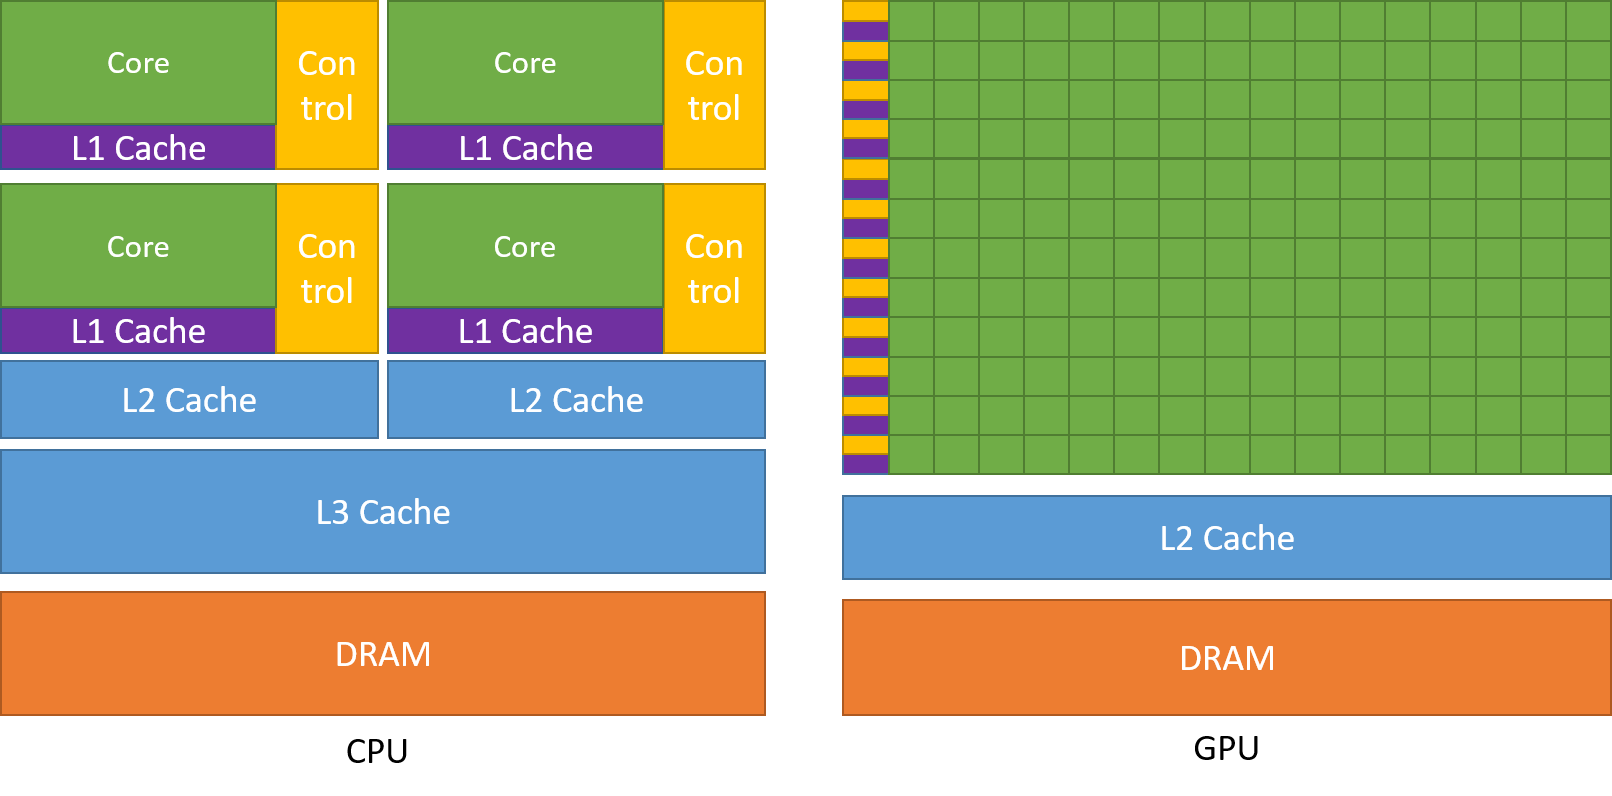
\includegraphics[width=0.8\linewidth]{Images/gpu-devotes-more-transistors-to-data-processing.png}
    \caption[GPU vs CPU transistor allocation for data processing.]{The GPU devotes 
more transistors to data processing than the CPU. Each (green) core acts as a thread 
that executes the same instruction on different data elements. Source: 
\cite{nvidia2025cuda}.}
    \label{fig:gpu-architecture}
\end{figure}        

A GPU executes a large number of lightweight threads (Figure 
\ref{fig:gpu-architecture}), organised into warps, groups of 32 threads that execute 
the same instruction simultaneously on a single streaming multiprocessor (SM). This 
single-instruction multiple-thread (SIMT) model maps directly onto operations such as 
FFTs, element-wise multiplication, and threshold comparisons, where the same 
computation is applied independently to many data elements. When threads within a warp 
follow different control flow paths — a condition known as warp divergence — the 
divergent branches must be executed serially, reducing parallelism (see Figure 
\ref{fig:warp-diverge}).

\begin{figure}
    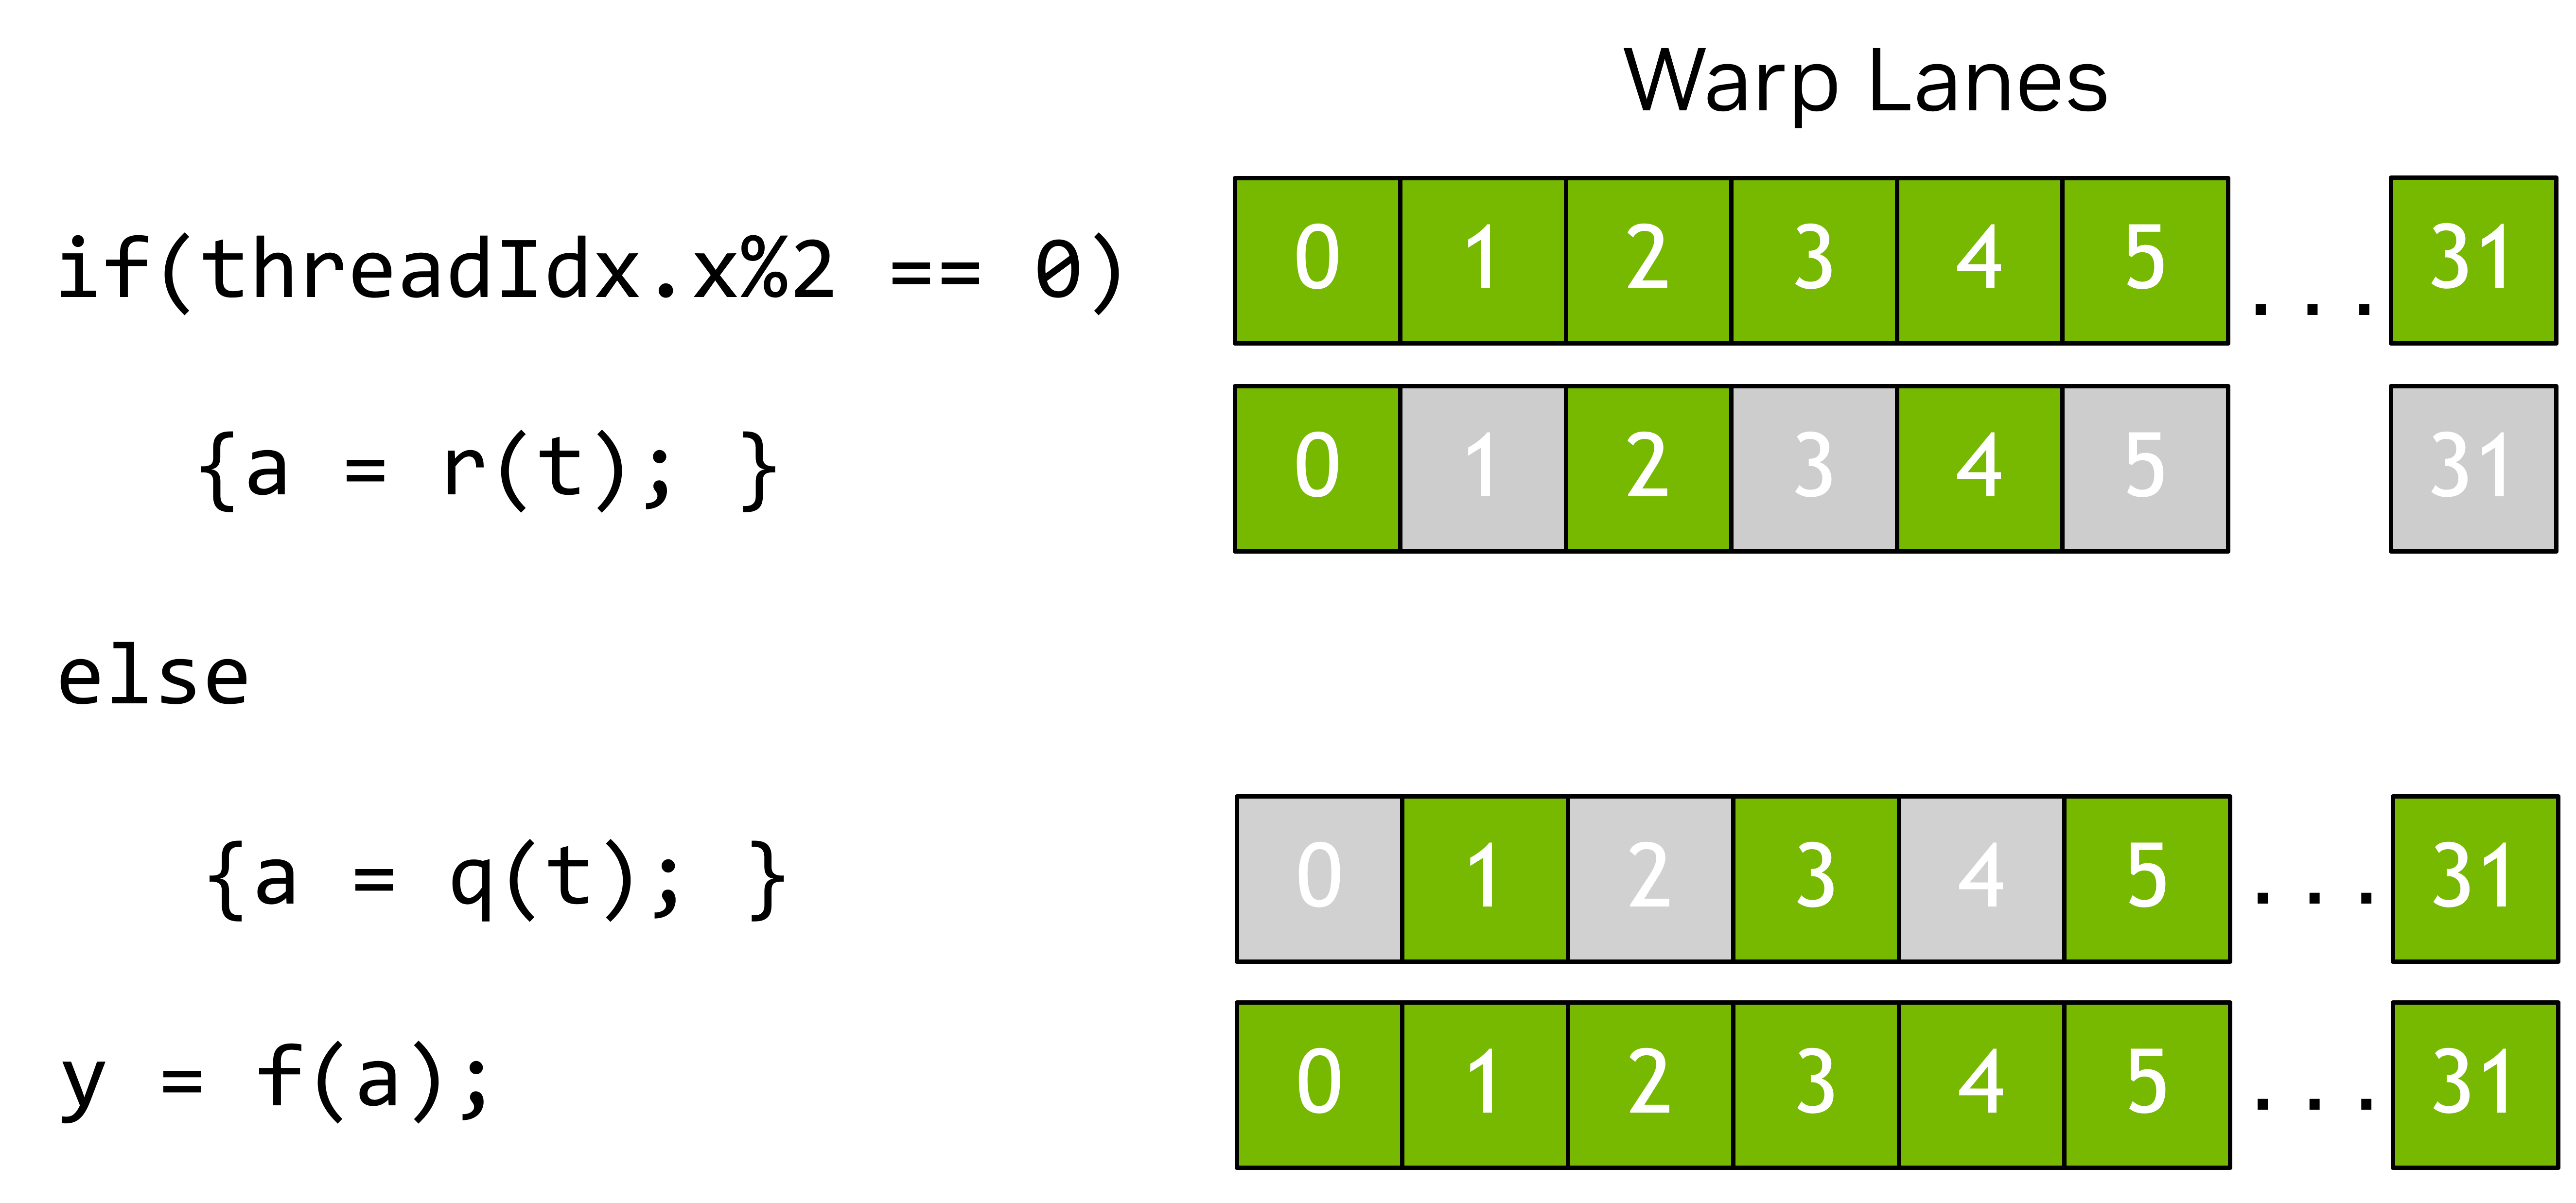
\includegraphics[width=0.8\linewidth]{Images/active-warp-lanes.png}
    \caption[Warp divergence causing serial execution of divergent branches.]{In this example, branching
    paths in execution between the even and odd threads prevent all threads from executing in parallel.
    All even threads execute the top branch while all odd threads are idle, then vice versa. As a result,
    the execution time is the sum of the two branches instead of the maximum. 
    Source: \cite{nvidia2025cuda}.}
    \label{fig:warp-diverge}
\end{figure}

Memory access patterns also affect throughput. Global memory is accessed most 
efficiently when threads in a warp read or write contiguous memory locations 
simultaneously, a pattern known as coalesced access. Non-coalesced access wastes
memory bandwidth by reading non-contiguous memory locations.
Figure \ref{fig:coalesced-access} illustrates one such situation. The warps will need 
to retrieve data from global memory more frequently when accessing non-contiguous 
memory. For this reason, ensuring that as much as possible of the data in each cache 
line fetched is actually used is an important part of performance optimisation of 
memory accesses on these devices.

\begin{figure}
    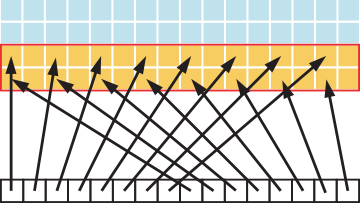
\includegraphics[width=0.5\linewidth]{Images/adjacent-threads-accessing-memory-with-stride-of-2.png}
    \caption[Non-coalesced memory access with stride of 2 reducing bandwidth efficiency.]{Figure 6:
    Adjacent threads (bottom) accessing every second memory location (orange). Since memory is cached in 
    large blocks,
    the large stride of 2 results in a 50\% reduction in load/store efficiency, since half of all cached
    memory is not being used. Source: \cite{nvidia2025cuda}.}
    \label{fig:coalesced-access}
\end{figure}

In discrete GPU systems, the CPU and GPU maintain separate physical memory pools 
connected by a bus such as PCIe, and data must be explicitly transferred between host 
and device memory. In system-on-chip (SoC) platforms such as the NVIDIA Jetson family, 
the CPU and GPU share the same physical DRAM. This is called physically shared memory. 
Both processors access the same physical addresses, and the memory subsystem handles 
coherency, eliminating the explicit transfer step.

Shared memory is a separate, small, low-latency scratchpad memory local to each SM, 
explicitly managed by the programmer. It allows threads within a thread block to 
exchange data and cache intermediate results without accessing global memory. It is 
used in GPU implementations of reductions, transpose operations, and tiled matrix 
multiplications, where threads cooperatively load a tile of data into shared memory and 
reuse it across multiple operations.